\chapter{Основные определения и математическая модель} \label{definitions}

\section{Некоторые сведения из теории графов}
Ниже даны основные определения из теории графов, которые используются в данной работе.

\emph{Простым невзвешенным графом} $G$ называется пара $(V,\ E)$, где $V$ это конечное множество вершин, а $E=V\times V$~--- множество (ориентированных) ребер. 
\emph{Матрицей смежности} графа $G$ называется матрица $A$, в которой $a_{ij}=1,$ если в графе $G$ есть ребро из вершины $i$ в вершину $j$, т.е. $(i,\ j)\in E.$ В противном случае $a_{ij}=0.$
Граф называется \emph{неориентированным}, если матрица $A$ симметрична, иначе --- \emph{ориентированным}. 

Говорят, что граф $G$ содержит \emph{исходящее остовное дерево}, если в нем существует подргаф $G_1=(V, E_1\subset E)$, такой что:
\begin{enumerate}
\item $G_1$ не содержит циклов.
\item В $G_1$ имеется вершина, от которой имеется путь до любой другой вершины в $H$.
\end{enumerate}

\emph{Степенью вершины} $i$ называется количество ребер $(i,\ j)$, т.е. ребер, исходящих из нее.
\emph{Матрицей степеней вершин} называется диагональная матрица $D$, в которой элементы $d_{ii}$ равны степени $i$-й вершины.

\begin{definition}
\emph{Матрицей Лапласа} графа $G$ определяется как $L=D-A,$ где $A$~---матрица смежности, а $D$~--- матрица степеней вершин.
\end{definition}

Матрица Лапласа обладает рядом интересных свойств, связанных со свойствами соответствующего графа. Некоторые из этих свойств:

\begin{itemize}
\item Для неориентированных графов $L$ симметрична, следовательно, ее собственные значения чисто действительные.
\item Действительные части собственных значений $L$ ограничены отрезком $[0;\ 2(|V|-1)]$ (следствие теоремы Гершгорина).
\item 0 является собственным значением матрицы Лапласа. Если граф содержит остовное исходящее дерево, то кратность 0 равна единице.
\end{itemize}

При изучении скорости сходимости к формации в сетевых моделях большую роль играет следующее определение.

\begin{definition}
\emph{Алгебраической связностью неориентированного графа} $G$ называется наименьшее ненулевое собственное значение его матрицы Лапласа $L$.
\end{definition}

В данной работе рассматриваются неориентированные невзвешенные графы, содержащие исходящее остовное дерево. Матрица Лапласа таких графов имеет собственное значение 0 кратности 1, все остальные собственные значения ненулевые и вещественные.

\section{Базовая модель консенсуса в графовой модели}

Базовая модель консенсуса описывает процесс схождения к консенсусу группы из $N$ агентов, обменивающихся информацией в соответствии с графом влияний $G$ с матрицей смежности $A$. У каждого агента есть вектор состояния $x_i$, и динамика системы описывается таким уравнением:
\begin{equation}
\label{eq:consensus}
\dot{x_i}(t)=-\sum_{i,j}a_{ij}\left(x_i(t)-x_j(t)\right)\ \ \ \ i=1,\ldots,N.
\end{equation}

Система схоится к консенсусу, когда $\exists x_f: \forall i,\ \forall x_i(0): x_i(t)\rightarrow x_f.$

Эта простейшая модель входит как составляющая часть в итоговое уравнение движения изучаемой модели.

Важный результат для базовой модели консенсуса:
\begin{theorem}
Система \ref{eq:consensus} сходится к консенсусу тогда и только тогда, когда граф влияний имеет остовное исходящее дерево. 
\end{theorem}

\section{Линейная модель движения в формации}
Исходная модель, взятая из работы \cite{veerman2005flocks} (будем далее называть ее "модель 1") описывает систему из $N$ агентов, движущихся в $d$-мерном пространстве (в рассматриваемом случае $d=2$). Перед агентами стоит следующая задача: начав движение из заданной позиции с заданными скоростями, выстроиться в заранее заданную формацию и продолжить движение в ней. 

Каждому агенту известна разница своих координат и скоростей с координатами и скоростями некоторых других агентов, которые входят в его \emph{множество соседей}. Эти множества задаются \emph{графом влияний} $G$, в котором проведено ребро $i\rightarrow j$, если агент $j$ получает информацию от агента $i$. Каждый агент знает также свою позицию в желаемой конфигурации и позиции его соседей.

Теперь опишем модель формально.
Состоянием $i$-го агента является  вектор $x_i$
в пространстве $\mathbb{R}^{2d}$:
$$x_i=x^p_i\otimes\veccol{1;0}+x^v_i\otimes
\veccol{0;1}.$$
Здесь $x^p_i$ и $x^v_i$ это пространственное положение и скорость агента, а $\otimes$\ ---\ произведение Кронекера.~\footnote{Таким образом, вектор $x_i$ имеет вид (для $d=2$): $\left(x_i, \dot{x}_i, y_i, \dot{y}_i\right)$. Обозначения позаимствованы из работы \cite{veerman2005flocks}.}

Состояние всей системы описывается вектором $x=\left(x_1,x_2,\ldots,x_N\right)^T$. Желаемая формация задается вектором 
$h={\left(h_1,0,h_2,0\ldots h_N,0\right)^T=h_p\otimes\left(1,0\right)}^T\in\mathbb{R}^{2dN}$.

\begin{definition}
\\\\
Говорят, что система движется \emph{в формации}, когда $\exists$ функции $q(t)$, $w(t)$, такие что:
$
x^p(t)-h^p\equiv q(t)\vec{1},\ x^v(t)\equiv w(t)\vec{1}.
$
\\
Говорят, что система \emph{сходится к формации}, когда
$
x^p(t)-h^p-q(t)\vec{1}\rightarrow 0,\ x^v(t)-w(t)\vec{1}\rightarrow 0.
$
\end{definition}

Смысл определения в том, что при движении в формации все агенты имеют одну и ту же скорость, а их позиции совпадают с требуемой формацией с точностью до некоторого смещения.

Уравнение движения агентов имеет в данной модели следующий вид: 
\begin{equation}
\dot{x_i}=A_1x_i+B_1u_i,
\end{equation} где
$$
A_1=\left( \begin{array}{cccc}
0 & 1 & 0 & 0 \\
0 & a_{22} & 0 & a_{24} \\
0 & 0 & 0 & 1 \\
0 & a_{42} & 0 & a_{44} \end{array} \right),\ \ \  
B_1=\[ \left( \begin{array}{cc}
0 & 0 \\
1 & 0 \\
0 & 0 \\
0 & 1 \end{array} \right),
$$
а $u_i$~--- это управляющий сигнал, который еще предстоит ввести. 

Вид матриц $A_1$, $B_1$ объяснен в работе \cite{veerman2005flocks}. Подматрица 
$A_0=\left( \begin{array}{cc}
a_{22} & a_{24} \\
a_{42} & a_{44} \end{array} \right)$ 
матрицы $A_1$ определяет динамику движения формации как целого. Числа $a_{24},\ a_{42}$ отвечают за кривизну траектории формации:

\begin{itemize}
\item При $a_{24}=-a_{42}\neq 0$ агенты двигаются в формации по окружности определенного радиуса; 
\item при $|a_{24}|\neq|a_{42}|,$ где $|a_{24}|,\ |a_{42}|>0$ ~--- по эллипсу;
\item при $a_{24}=a_{42}=0$~--- по прямой. 
\end{itemize}

Числа $a_{22}$ и $a_{44}$ отвечают за ускорение формации вдоль линии текущего курса:  при $a_{22}>0,\ a_{44}>0$ ускорение положительное, при $a_{22},\ a_{44}~$ --- отрицательное. 

В дальнейшем ограничимся случаем движения по прямой и по окружности, введя вместо $a_{24},\ a_{42}$ один параметр $k=a_{24}=-a_{42}$ --- кривизна траектории движения. При $k=0$ получаем прямолинейное движение, а по мере увеличения $k$ движение происходит по окружности все меньшего радиуса.

\begin{figure}[h]
  \begin{minipage}[h]{0.32\linewidth}
    \center{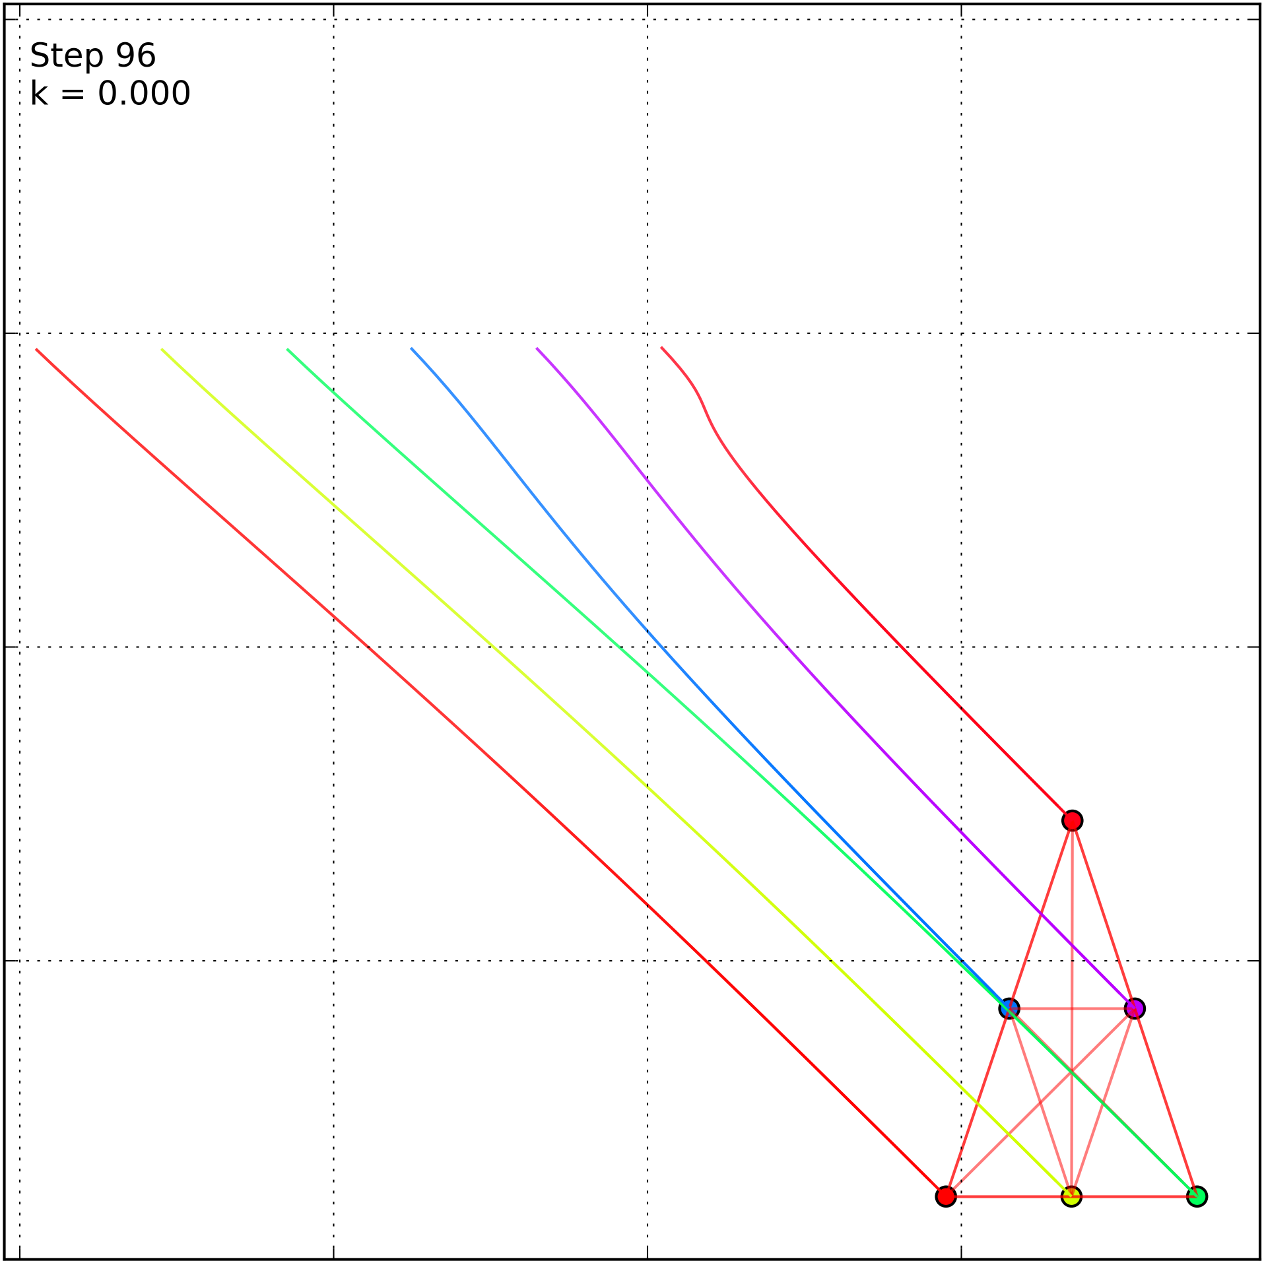
\includegraphics[width=\linewidth]{linear_straight.png} \\ а)}
  \end{minipage}
  \hfill
  \begin{minipage}[h]{0.32\linewidth}
    \center{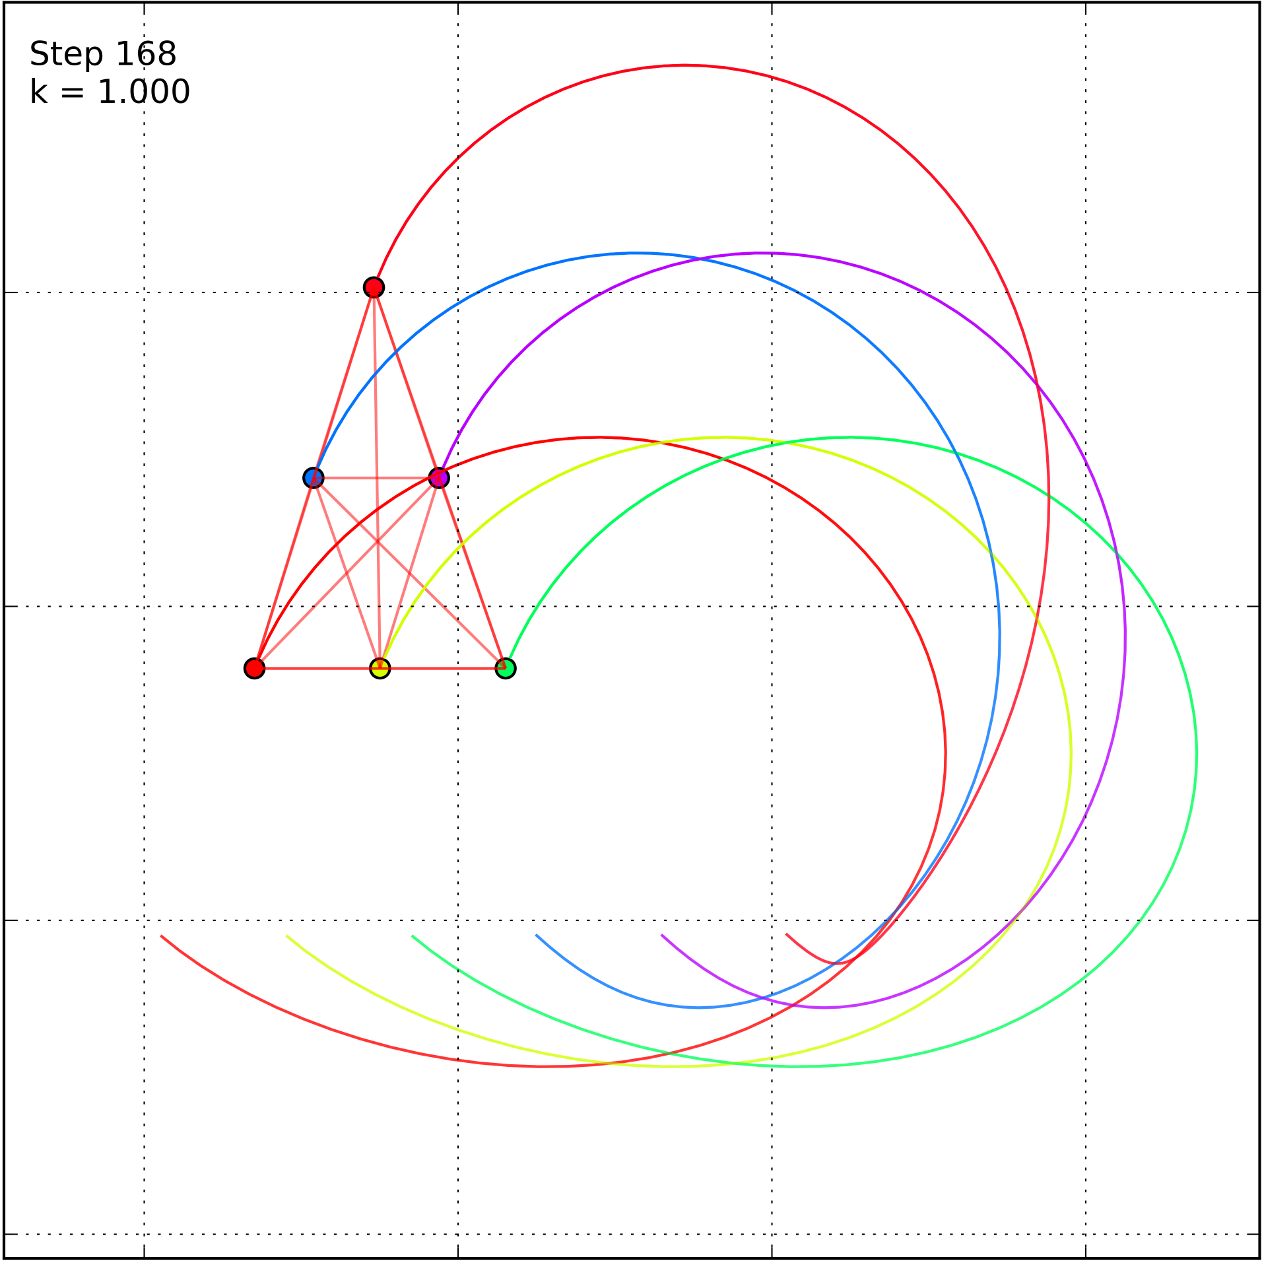
\includegraphics[width=\linewidth]{linear_circle.png} \\ б)}
  \end{minipage}
   \hfill
  \begin{minipage}[h]{0.32\linewidth}
    \center{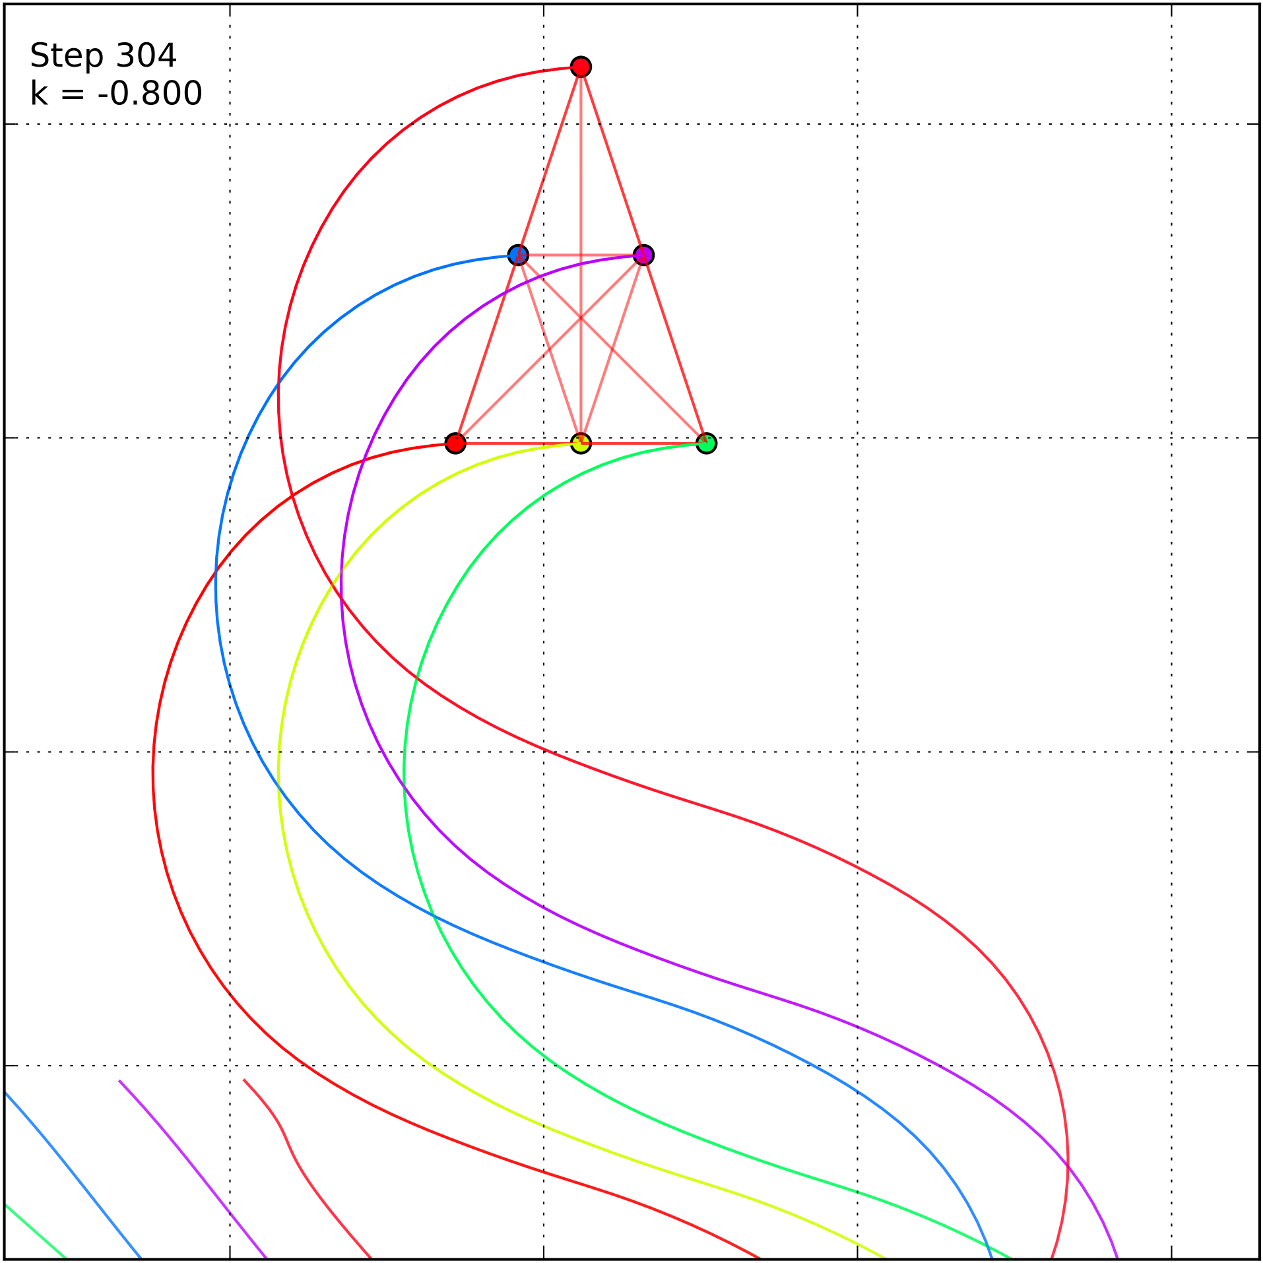
\includegraphics[width=\linewidth]{linear_variable_k.png} \\ в)}
  \end{minipage}
  \caption{Движение, задаваемое моделью 1. На рисунке a) параметр кривизны движения $k=0$, на рисунке б) $k=1$, на рисунке в) параметр $k$ меняет значение во время движения. Во всех случаях граф влияний полный, $f_1=f_2=-2.5$. Иллюстрации сделаны в интерактивном режиме симулятора модели.}
\label{fig:linear-motion}
\end{figure}

Управляющий сигнал получается преобразованием $u=Fz$, где $F$~--- матрица обратной связи, а $z$~---функция, описывающая "выходной сигнал" из системы. Этот выходной сигнал рассчитывается так же как и в базовой модели консенсуса:
$$
z_i=(x_i-h_i)+\frac{1}{|\mathbb{J}_i|}\sum_{j\in\mathbb{J}_i}\left((x_i-h_i)-(x_j-h_j)\right)\ \ \ \ i=1,\ldots,N.
$$

Объединив уравнения для всех агентов в одно, получим общее уравнение движения для всей системы:
\begin{equation}
\dot{x}=Ax+BFL(x-h),
\label{eq:linear-motion}
\end{equation}
где $L\equiv L_G\otimes I_{2N},\ L_G$~---матрица лапласа графа влияний $G$, а матрицы $A,\ B$ и $F$ определены через "размножение" матриц $A_1,\ B_1$ и $F_1$ для одного агента: $A=I_N\otimes A_1,\ B=I_N\otimes B_1, F=I_N\otimes F_1$, т.к. законы движения всех агентов одинаковы.

В работах \cite{lafferriere2005decentralized, veerman2005flocks} авторы ограничиваются матрицей обратной связи $F_1$ вида 
$$F_1=\left( \begin{array}{cccc}
f_1 & f_2 & 0 & 0 \\
0 & 0 & f_1 & f_2 \end{array} \right),$$ такая же матрица используется и в данной работе.

Для рассмотренной модели имеется ряд доказанных теоретических результатов, интересующие нас приведены ниже. 

Во-первых, так же как и в базовой модели консенсуса, существует необходимое условие сходимости модели:
\begin{proposition}
Необходимым условием сходимости модели к формации является наличие в графе влияний $G$ остовного исходящего дерева.
\end{proposition}

Но для рассматриваемой модели это условие не является достаточным. Достаточные условия сходимости даются следующей теоремой \cite{veerman2005flocks,lafferriere2005decentralized}:

Во-вторых, для случая неориентированных графов в работе \cite{lafferriere2005decentralized} имеется теорема о скорости сходимости к формации.
\begin{theorem}
Модель 1 сходится к формации, когда коэффициенты обратной связи $f_1,\ f_2$ и параметр $k$ удовлетворяют неравенствам 
\begin{equation}
\frac{{f_2}^2}{f_1}< -\frac{\beta^2}{\alpha(\alpha^2+\beta^2)}\ \ \text{и}
\end{equation}
\begin{equation}
|k|<\frac{-f_1|\beta|}{f_2\alpha}-\frac{f_2(\alpha^2+\beta^2)}{|\beta|},
\end{equation}
где $\alpha+i\beta=\lambda$~--- собственные числа матрицы Лапласа графа влияний $G$.
\end{theorem}

\begin{theorem}
Для неориентированных графов скорость сходимости пропорциональна выражению 
$(a_22+\lambda_1 f_2)/2,$ где $\lambda_1$~--- наименьшее ненулевое собственное значение матрицы $L_G$.
\end{theorem}

\section{Нелинейная модель движения в ориентированной формации}
Как можно видеть на рисунке \ref{fig:linear-motion}, формация не меняет своей ориентации при поворотах, что не очень реалистично. Изменив уравнение движения \ref{eq:linear-motion}, получим уже нелинейную модель 2:
\begin{equation}
\dot{x}=Ax+BFL(x-T_x h),
\label{eq:orientable-motion}
\end{equation}
где оператор $T_x$ определен как
\begin{equation}
T_x:h\rightarrow \sum^N_{i=1}E_i\otimes R_{x^v_i}\otimes
\left( 
\begin{array}{cc}
1 & 0 \\
0 & 0 \end{array} \right) h_i.
\end{equation}
В этом определении $E_i$ это матрица, состоящая из нулей и единственной единицей на $i$-й диагональной позиции, а $R_v:\mathbb{R}^2\rightarrow\mathbb{R}^2$ поворачивает базисный вектор $e_1$ в направлении вектора $v$.

Модель значительно усложнилась: перестала быть линейной и от агентов стало требоваться знать не только скорости относительно соседей, но и их собственные асболютные скорости. Следует также заметить, что $R_v$ не определен для нулевых векторов $v$, и поэтому модель 2 не допускает нулевой скорости агентов.

На рисунке \ref{fig:linear-motion-1} показаны траектории агентов в модели 2:

\begin{figure}[h]
  \begin{minipage}[h]{0.45\linewidth}
    \center{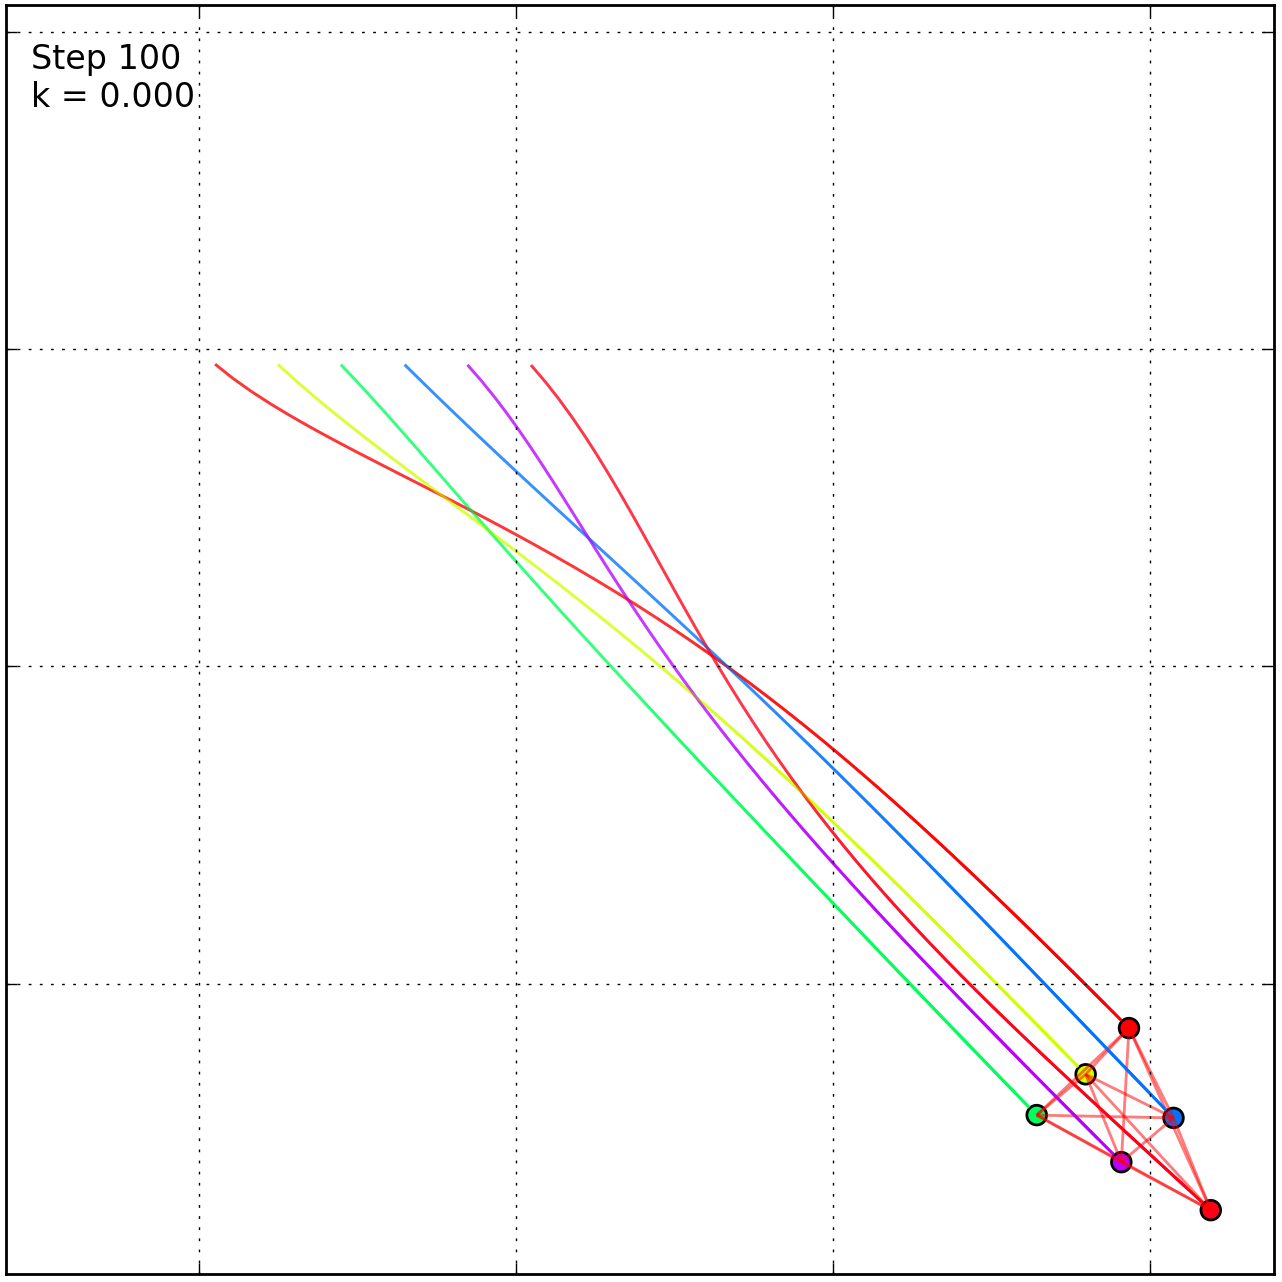
\includegraphics[width=\linewidth]{orientable_straight.png} \\ а)}
  \end{minipage}
  \hfill
  \begin{minipage}[h]{0.45\linewidth}
    \center{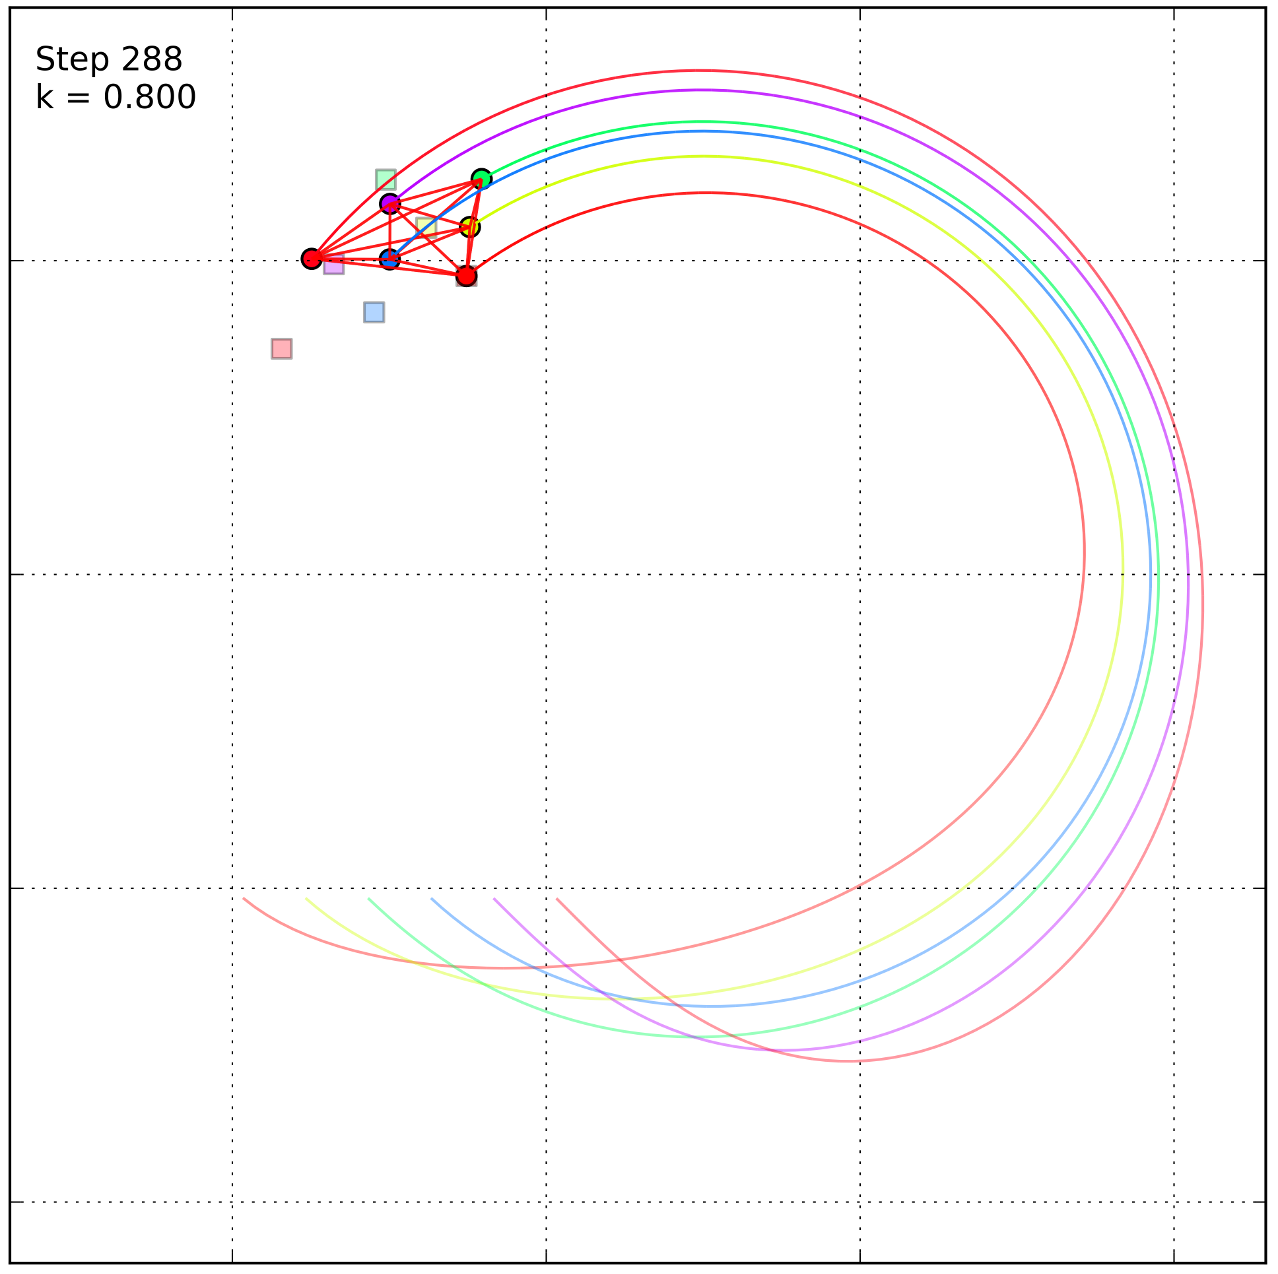
\includegraphics[width=\linewidth]{orientable_circle.png} \\ б)}
  \end{minipage}
  \caption{Движение, задаваемое моделью 2 --- формация ориентируется по направлению движения. На рисунке б) видно искажение формации во время совершения разворота.}
\label{fig:orientable-motion}
\end{figure}

На последнем рисунке видно, что во время разворота агенты выстраиваются не в точности в заданную формацию (на рисунке отмечена квадратами), а в ее немного искаженную версию. Причем при уменьшении радиуса разворота это искажение все больше. Этот факт приводит к тому, что становится сложнее формально определить условия, когда модель "сошлась к формации". Один из возможных подходов, который используется в данной работе, описан в разделе \ref{section:formation-measurement}.

\section{Дальнейшие расширения модели}
В этой работе в модель 2 были внесены еще две поправки. Получившуюся модель назовем моделью 3~--- именно она  рассматривается в данной работе. Рассмотрим эти поправки по очереди.

\subsection{Избегание столкновений}
Во-первых, чтобы избежать столкновений между агентами, в уравнение движения был добавлен потенциал отталкивания. Этот потенциал включается тогда, когда расстояние между агентами становится меньше заданного порога $r_0$ и линейно возрастает по ммере уменьшения расстояния. Чтобы не допустить возникновения бесконечно больших ускорений, его вклад в ускорение агентов ограничен параметром $r_1$, начиная с которого потенциал перестает возрастать. Интенсивность расталкивания регулируется параметром $D$.

Вид дополнительных ускорений, вызванных потенциалом расталкивания и действующих на агента $i$:
\begin{equation}
a^{rep}_i=-D\sum_{i\neq j,\\|r_{ij}|<r_0}}\min{\left(r_1,r_0-|r_{ij}|\right)\frac{r_{ij}}{|r_{ij}|}}.
\end{equation}

Рассмотренный потенциал отталкивания взят из работы \cite{vasarhelyi2014outdoor}, где он использовался для предотвращения столкновений между квадрокоптерами во время построения ими формации.

\subsection{Учет ненадежности связей в графе влияний}
Вторым дополнением модели послужил учет случайных разрывов связей в графе влияний, которые почти наверняка будут иметь место при построении реальных многоагентных систем.

Моделирование разрыва связей можно провести по-разному. Например, можно было моделировать разрывы и восстановления связей различными случайными процессами в зависимости от дополнительных предположений, например, пуассоновскими процессами с разными параметрами для разрыва и восстановления. В этой работе использовался более простой подход: при пошаговом
численном решении уравнения движения на каждом $k$-м шаге проводится обновление графа влияний. При этом для каждого ребра независимо решается с вероятностью $p$, будет ли оно деактивировано (т.е. не влиять на формирование множеств соседей) на протяжении следующих $k$ шагов. После $k$ шагов процедура повторяется.

Окончательная форма уравнения движения в модели 3 будет такой:
\begin{equation}
\dot{x}=Ax+BFL(t)(x-T_x h)+a^{rep}\otimes \veccol{0;1}.
\end{equation}

\section{Определение меры близости к формации}
\label{section:formation-measurement}

Для оценки того, насколько близка система к формации, используется следующий подход:
для двух соседних шагов симуляции рассчитывается векторы разницы между текущей конфигурацией агентов в пространстве координат и желаемой формацией. Эти векторы вычисляются с поправкой на текущую ориентацию формации и ее общее смещение всех агентов относительно начала координат. Это достигается смещением всех векторов агентов на координаты первого агента с последующим поворотом на угол текущей средней скорости формации:

\begin{equation}
z_{cur}=(x_i-x_0)R_{v_{avg}}.
\end{equation}

Затем разность получившихся векторов делится на количество агентов и длину шага симуляции. От получившегося вектора берется норма, которая и принимается за меру качества формации:

\begin{equation}
\Delta=\frac{||z_{cur}-z_{prev}||}{N\tau}.
\end{equation}

Эта мера стремится к нулю когда прекращается относительное движение агентов, с учетом их общего смещения и ориентации.

На рисунке \ref{fig:formation-error} показаны графики меры близости системы к формации в зависимости от времени:

\begin{figure}[h]
  \begin{minipage}[h]{0.45\linewidth}
    \center{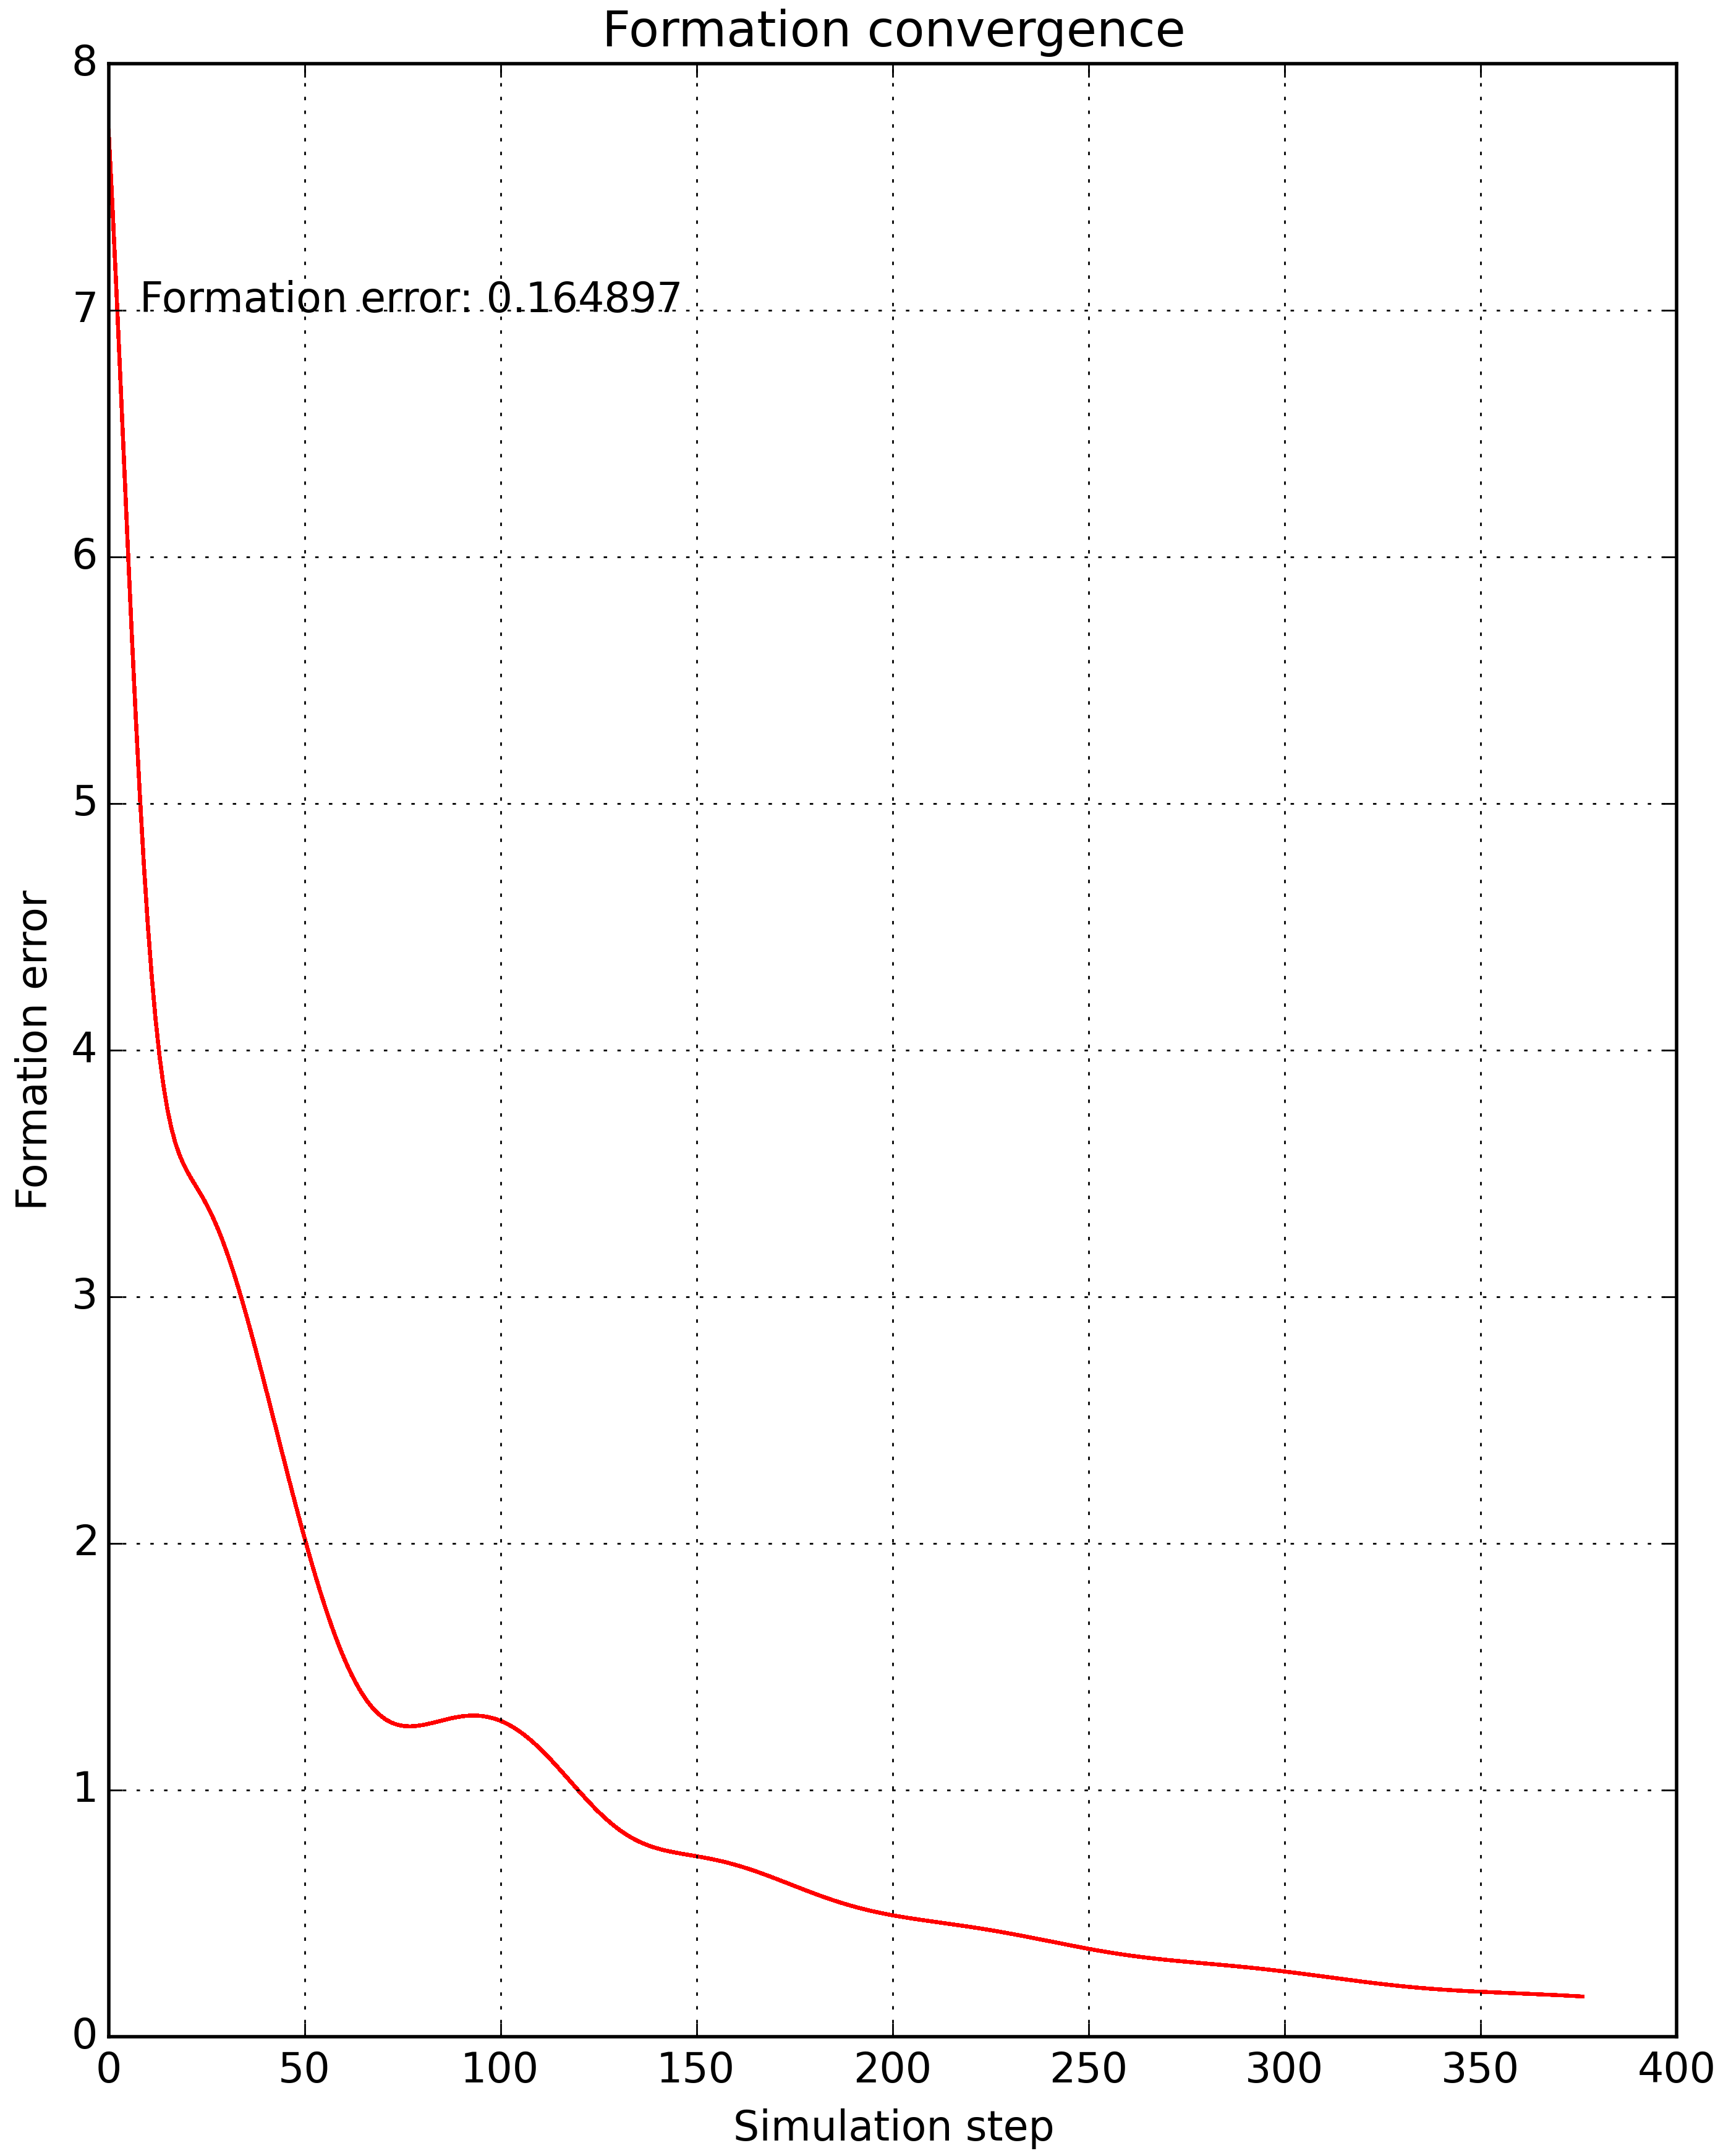
\includegraphics[width=\linewidth]{formation_error_chart_d_0.png} \\ а)}
  \end{minipage}
  \hfill
  \begin{minipage}[h]{0.45\linewidth}
    \center{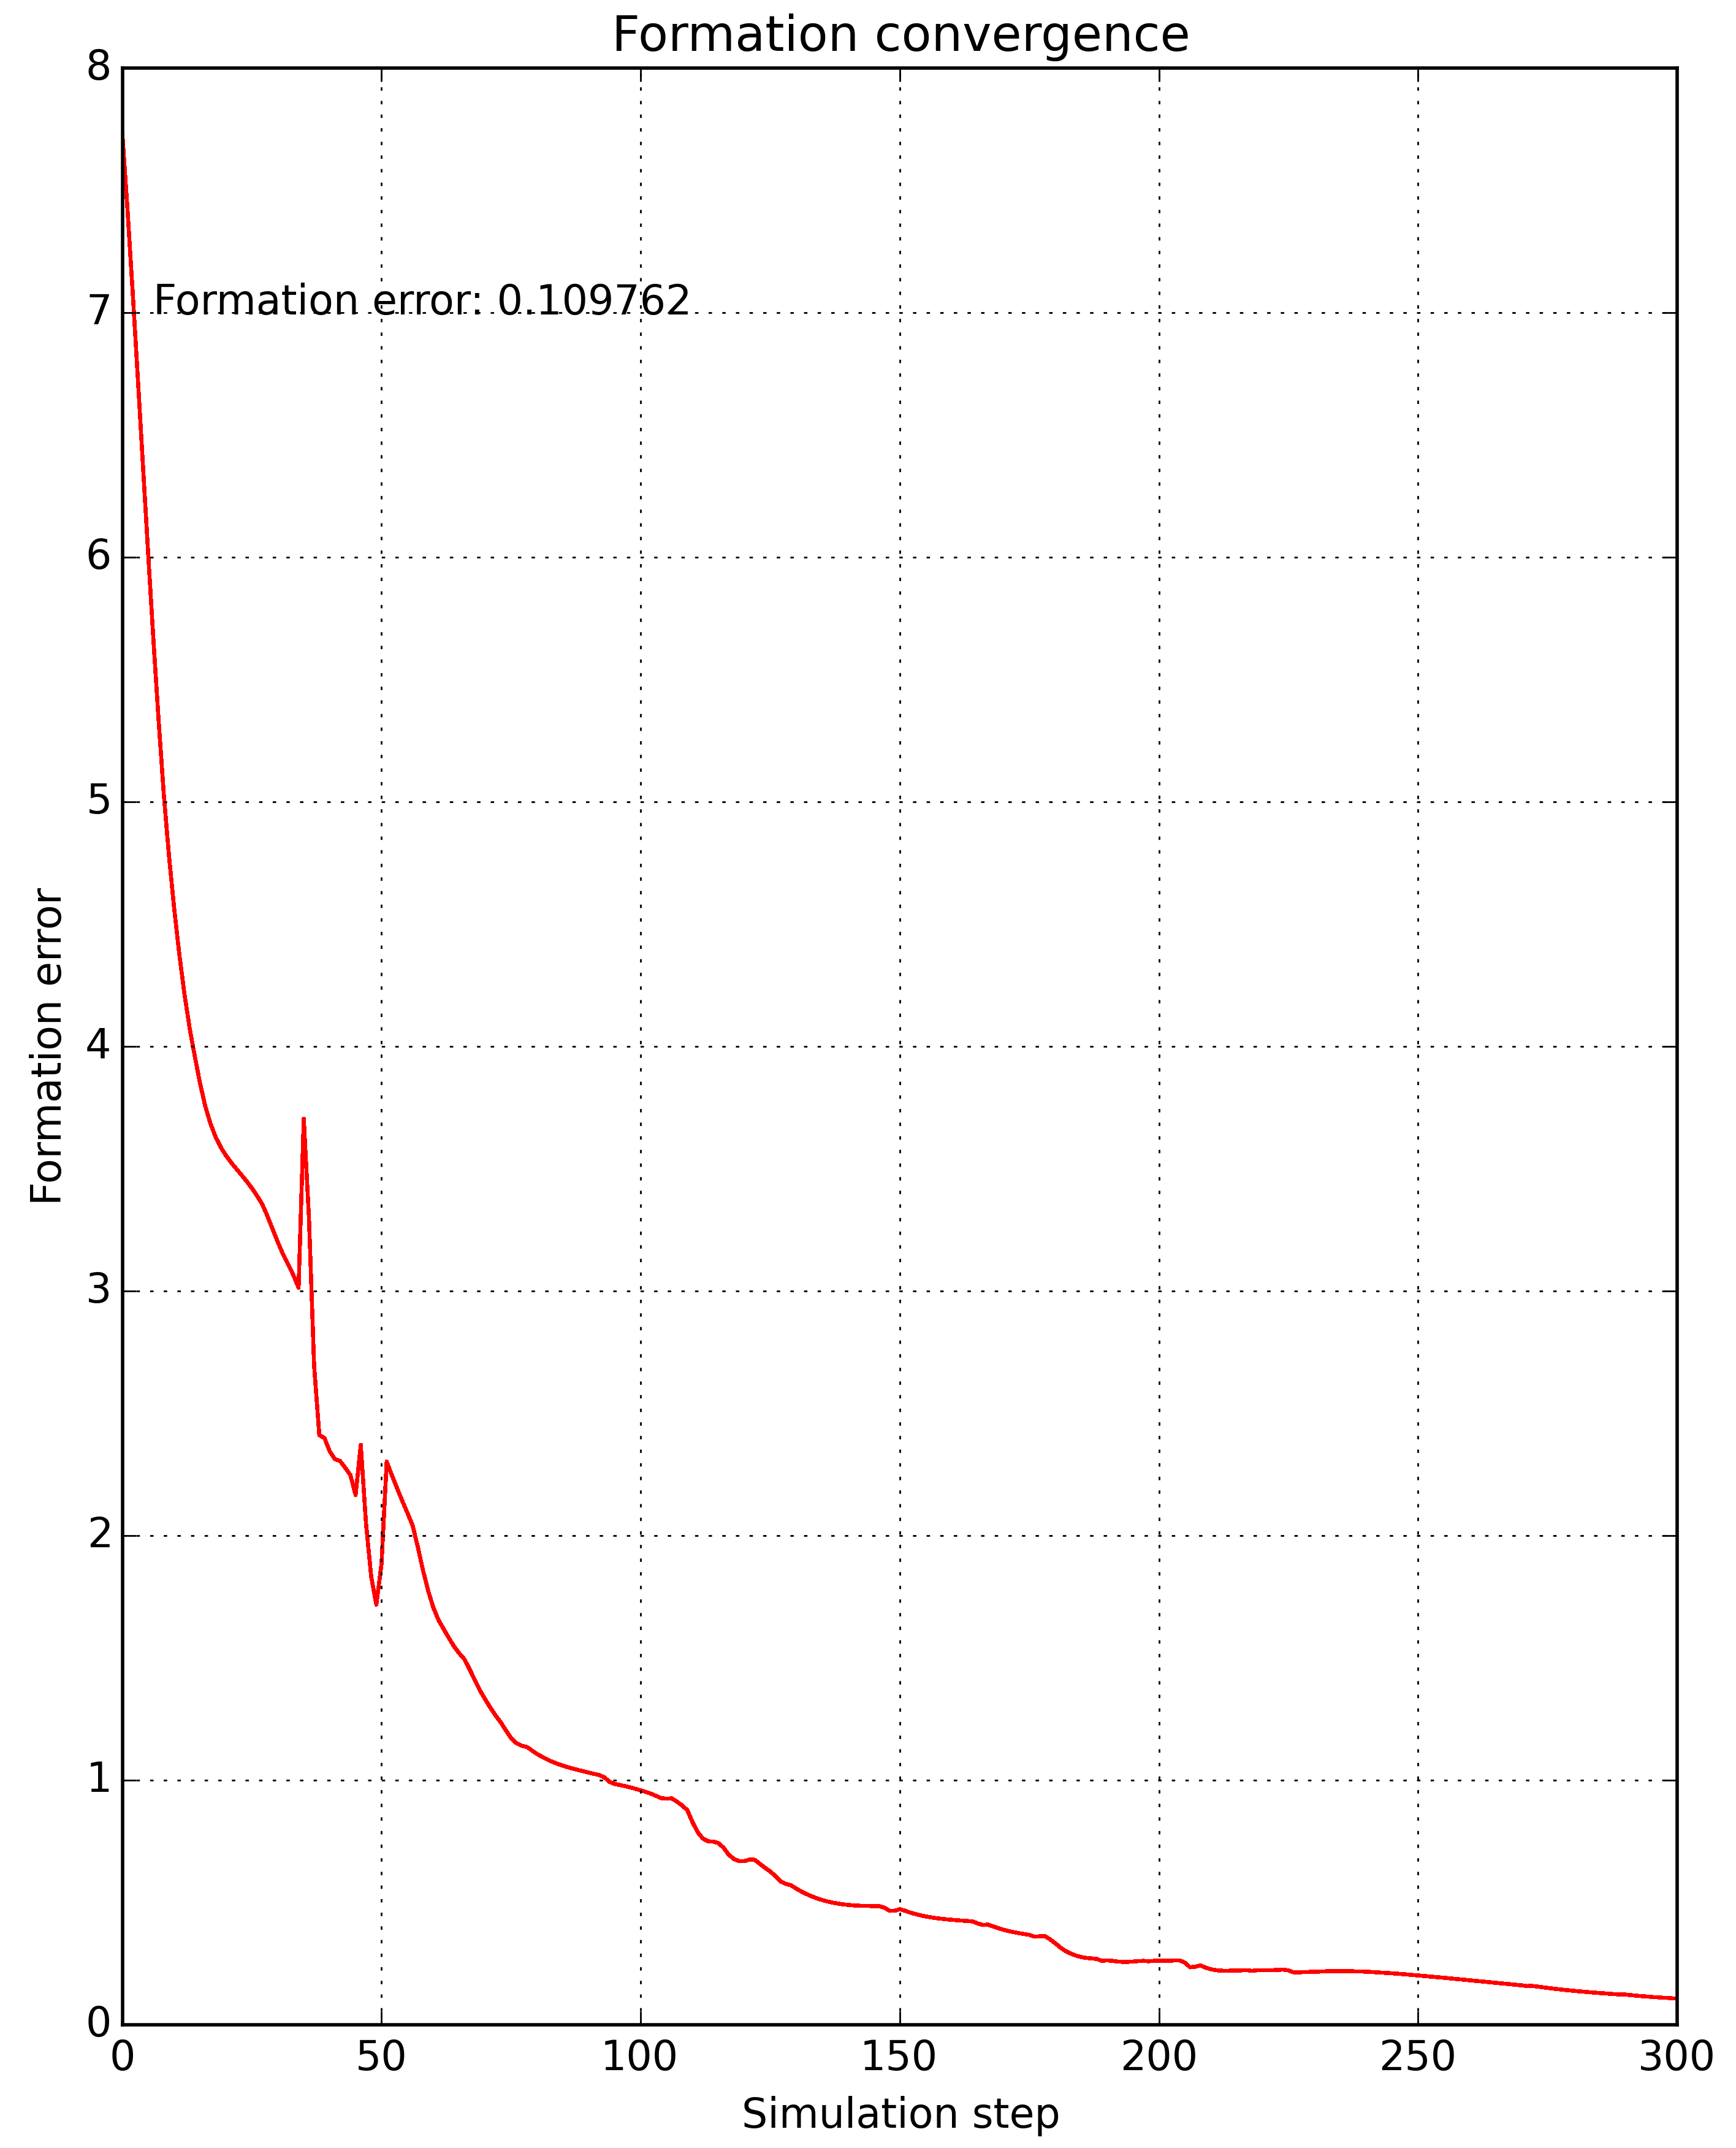
\includegraphics[width=\linewidth]{formation_error_chart_d_1e3.png} \\ б)}
  \end{minipage}
  \caption{На рисунке а) показан случай без отталкивания ($D=0$), на рисунке б)~--- с отталкиванием, ($D=1000$), все прочие условия одинаковы. В данном случае отталкивание помогло не только избежать столкновений, но и добиться быстрейшей сходимости к формации.}
\label{fig:formation-error}
\end{figure}


\clearpage
